\documentclass[12pt,a4paper]{article}
\usepackage{graphicx}
\usepackage[margin=1in]{geometry}
\usepackage[table,xcdraw]{xcolor}
\usepackage{float}
\usepackage[utf8]{inputenc}
\usepackage[english]{babel}
\usepackage{chemfig}
\usepackage[backend=biber,style=numeric]{biblatex}
\restylefloat{table}
\usepackage[T1]{fontenc}
\usepackage{amsfonts}
\usepackage{subcaption}
\usepackage{csquotes}
\usepackage[utf8]{inputenc}
\usepackage[english]{babel}
\usepackage{blindtext}
\usepackage{amssymb}
\usepackage{amsthm}
\usepackage{amsmath}
\renewcommand\qedsymbol{QED}
\addbibresource{hanoi\_cite.bib}
\title{Investigation on the Tower of Hanoi}
\author{Je-Yu Leo Chou }
\date{April 4th 2021}

\begin{document}
	\maketitle
	\tableofcontents
	\section{Introduction}
	\begin{figure}[ht]
		\begin{center}
			\includegraphics[width=\linewidth]{Tower_of_Hanoi.jpeg}
			\caption{A model of the Tower of Hanoi with 8 disks, and 2 additional, empty rods. Created in 2005 by user Ævar Arnfjörð Bjarmason and shared under the CC BY-SA 3.0 license}
		\end{center}
	\end{figure}
	\subsection{History of the Tower of Hanoi}
	The tower of Hanoi is a mathematical puzzle invented by a French mathematician named Édouard Lucas in the 19th century \cite{Buddies}. It was said that if one follows the assigned rule for 64 disks, the time to complete the task would mean the end of the world (there is also another legend in which this is  a test for young priest in hindu temples) \cite{Buddies}.
	\subsection{Problem Statement}
	The tower of Hanoi is a simple, iterative mathematical puzzle involving three diagrams \cite{Buddies}. At the start, there is an arbitrary amount of disks placed at the first peg with two additional empty pegs as shown in figure 1.  \newpage
	\noindent The problem is simple: Move all disk from the first pole to the third pole \cite{Buddies}. There are, however, two additional rules: (a) you may only move one disk at a time, and (b) the smaller disk must be on top of a larger disk \cite{Buddies}. Figure 2 is the minimal move solution for 3 disks.\newline
	\begin{figure}
		\begin{center}
			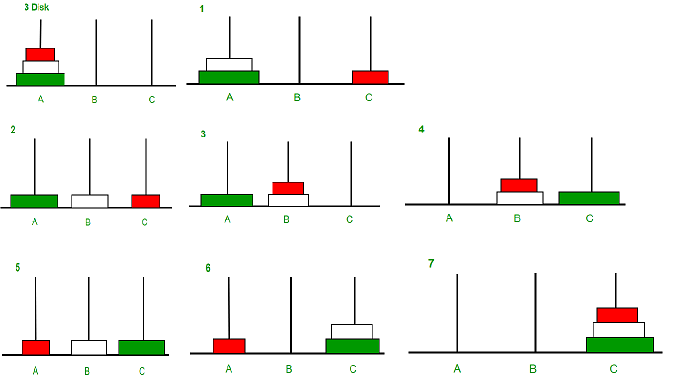
\includegraphics{3-disk.png}
			\caption{A method to solve the puzzle with 3 disks. Note that this fashion requires the minimal amount of moves of seven moves. This image, and its original article, was on GeeksforGeeks, contributed by Rohit Thapliyal, and shared under the CC BY-SA 3.0 license}. 
		\end{center}
	\end{figure}
	\subsection{Motivation}
	The tower of Hanoi is a longstanding problem that is often presented to older kids as well as programmers as the problem itself isn't hard and is an iterative problem (the same set of instruction is used over and over again) \cite{Buddies}. This famous puzzle was presented to me multiple times throughout my schooling, yet I never saw the real world significance of it. However, as a high schooler and a programmer now, I saw the application of it in many types of problems and its importance, as recursion has proven useful in many disciplines, such as creating tries and solving other famous mathematical puzzles such as Knight's Moves Problem. 
	
	\section{Investigation}
	\subsection{Finding a Pattern}
	In order to investigate the minimal move (thus the most efficient algorithm) for this problem, it is important to find a patterns in which to solve the problem. To find it, we will run through some cases in order to establish its relation. More specifically, we will be looking at cases where n=1; n=2; n=3, and finally when n=k where n is the number of disks and k $\in \mathbb{N}$. Below, A, B, and C will refer to the three pegs individually, where peg A is the peg with all the disks at the start, peg B is the helper peg, and peg C is the final peg where all disk should go in the end. 
	\subsubsection{n=1}
	This is the most trivial case, and one that will become important later. To do this, all we need to do is the move disk one from A to C
	\subsubsection{n=2}
	In this case, there are a minimal of three steps to take, as listed:
	\begin{enumerate}
		\item Move disk 1 from A to B
		\item Move disk 2 from A to C
		\item Move disk 1 from B to C
	\end{enumerate}
	\subsubsection{n=3}
	This is the case where the pattern starts to emerge. We first examine the seven steps required:
	\begin{enumerate}
		\item Move disk 1 from rod A to rod C
		\item Move disk 2 from rod A to rod B
		\item Move disk 1 from rod C to rod B
		\item Move disk 3 from rod A to rod C
		\item Move disk 1 from rod B to rod A
		\item Move disk 2 from rod B to rod C
		\item Move disk 1 from rod A to rod C
	\end{enumerate}
	These steps are represented visually in Figure 2. From this, we can see a clear pattern where in order to move all three disks, we first have to first n-1 disks to a separate, auxiliary peg, then move the final disk to the final peg, then move the n-1 disks from the auxiliary peg to the final peg. This brings us to the n=k scenario
	\subsubsection{n=k}
	As mentioned before, in order to solve for an arbitrary amount of pegs, there are only four steps to follow:
	\begin{enumerate}
		\item Move $k-1$ pegs to the auxiliary peg
		\item Move the $k^{th}$ peg to the final peg
		\item Move the $k-1$ pegs from the auxiliary peg to the final peg
	\end{enumerate}
	This is an iterative problem in mathematics that can be solved with recursion. Recursion refers to solving a problem by first solving a smaller version problem until reaching a trivial point, where the function stops calling on itself. This can be seen from the previous steps \cite{recursion}. 
	\subsection{Finding an Expression}
	To find the minimal moves required to solve the problem, the following table was created:
	% Please add the following required packages to your document preamble:
	% \usepackage{graphicx}
	% \usepackage[table,xcdraw]{xcolor}
	% If you use beamer only pass "xcolor=table" option, i.e. \documentclass[xcolor=table]{beamer}
	\begin{table}[H]
		\centering
		\title{Table 1: Comparision on minimum steps with the number of disks}
		\resizebox{\textwidth}{!}{%
			\begin{tabular}{rrrllll}
				\rowcolor[HTML]{FCE5CD} 
				\multicolumn{1}{l}{\cellcolor[HTML]{F4CCCC}Number of Disks} & \multicolumn{1}{l}{\cellcolor[HTML]{C9DAF8}Minimum Steps} & \multicolumn{1}{l}{\cellcolor[HTML]{FCE5CD}Difference} \\
				\rowcolor[HTML]{FFFFFF} 
				0                                                           & 0                                                         & N/A                                                     \\
				\rowcolor[HTML]{FFFFFF} 
				1                                                           & 1                                                         & 1                                                       \\
				\rowcolor[HTML]{FFFFFF} 
				2                                                           & 3                                                         & 2                                                       \\
				\rowcolor[HTML]{FFFFFF} 
				3                                                           & 7                                                         & 4                                                       \\
				\rowcolor[HTML]{FFFFFF} 
				4                                                           & 15                                                        & 8                                                       \\
				                              
			\end{tabular}%
		}
	\end{table}
	In order to come up with an equation to find out what the equation is for the minimal moves required for n disks, this investigation offers its examination along with its proof. \newpage
	\subsubsection{Graphs}
	\begin{figure}[ht!]
		\begin{subfigure}{.55\textwidth}
			\includegraphics[width=\linewidth]{scatter_plot.png}
			\caption{scatter plot of disks vs moves}
			\label{fig:fig1}
		\end{subfigure}%
		\begin{subfigure}{.55\textwidth}
			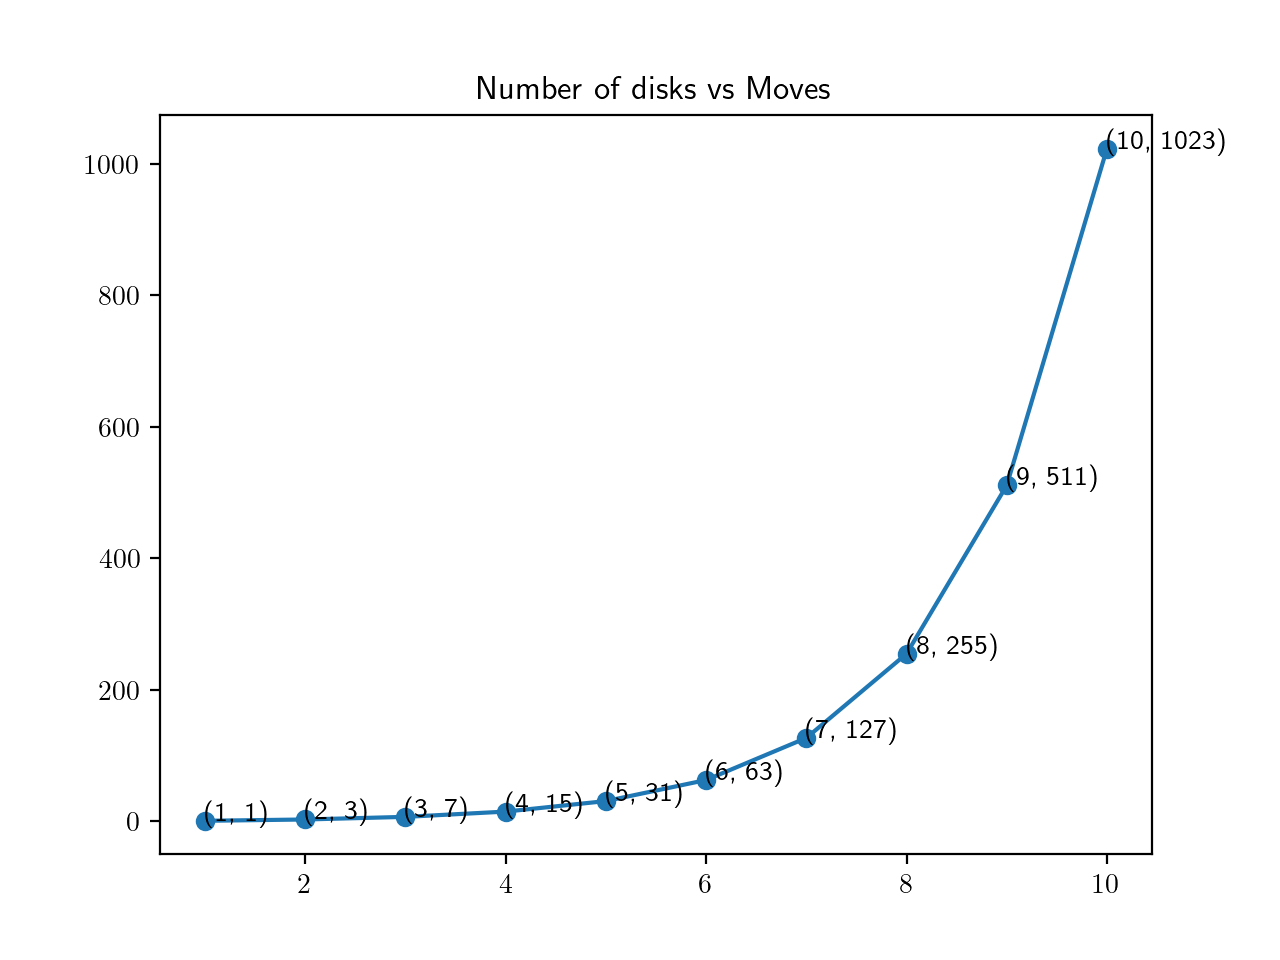
\includegraphics[width=\linewidth]{Figure_1}
			\caption{Fit of a line over the scatter plot}
			\label{fig:sfig2}
		\end{subfigure}
	\caption{Tracing out the graph of disks vs moves through first a scatter plot then a fit, graphed with \cite{matplotlib}}
	\label{fig1:fig1}
	\end{figure}
	\begin{figure}[h!]
		\begin{subfigure}{.55\textwidth}
			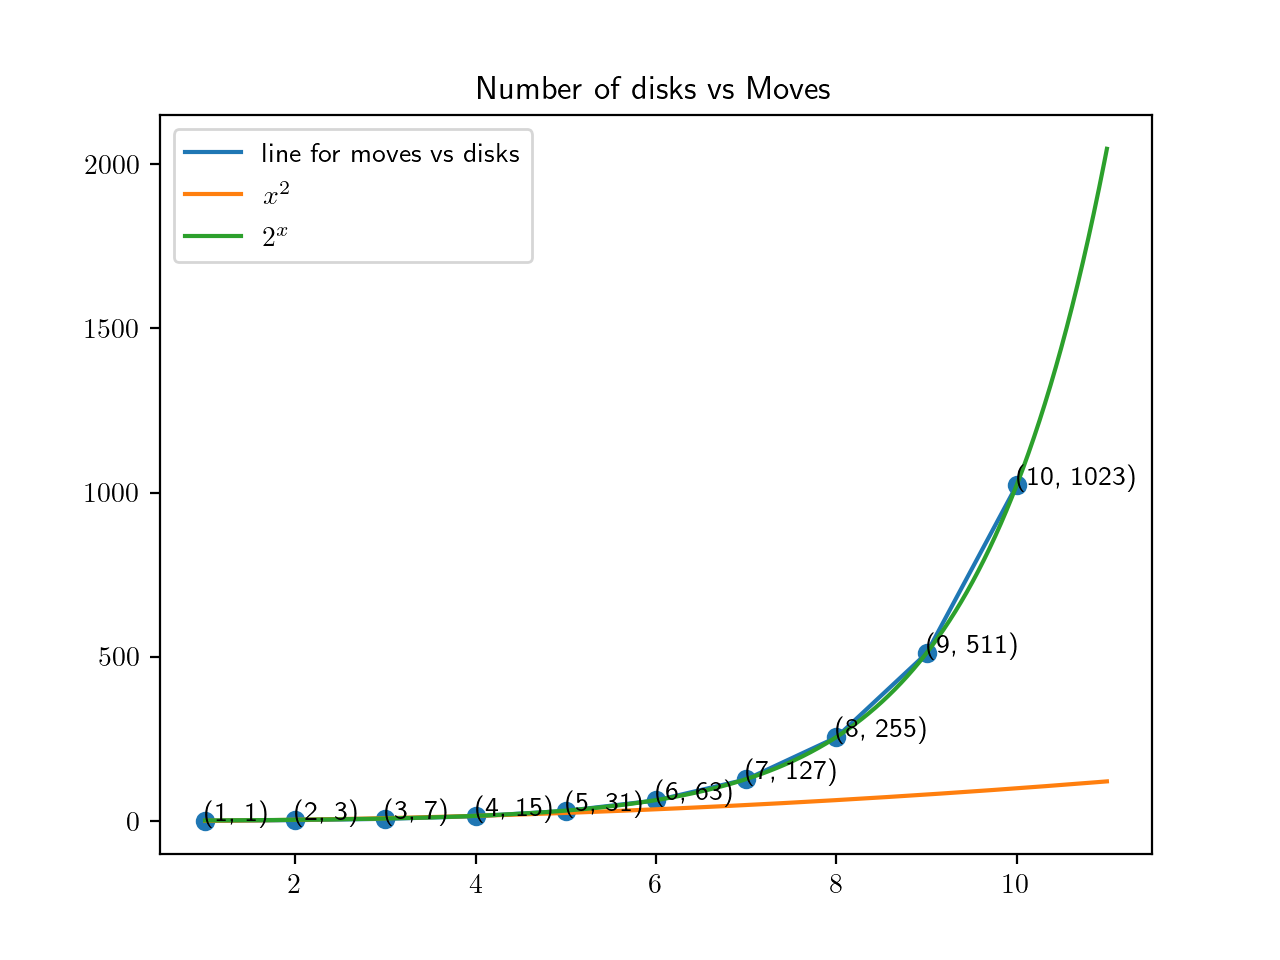
\includegraphics[width=\linewidth]{comparision.png}
			\caption{Graphs of $x^2$ and $2^x$ plotted along the original plot}
			\label{fig:fig3}
		\end{subfigure}
	\begin{subfigure}{.55\textwidth}
		\includegraphics[width=\linewidth]{zoomed_in.png}
		\caption{Zoomed in version for the disks vs moves graphs as well as the line for $2^x$}
		\label{fig:fig4}
	\end{subfigure}
	\caption{Different graphs to establish the relationship between disks and its required moves, as well as other functions to better understand the exponential relationship, graphed with \cite{matplotlib}}
	\label{fig:fig}
	\end{figure}
	As seen from Table 1, there is a constant difference between the current term and its preceding term, hinting towards an exponential relationship. Graphically, we can also see it tracing out an exponential pattern, as seen from figure 3 plots a and b. \newline
	Finding the exponential relationship isn't enough though, as $x^2$ and $2^x$ are still both valid assumptions as the difference is always an even number. In order to better investigate this, I plotted the graphs of $x^2$ and $2^x$ alongside the original scatter plot. As demonstrated from figure 4a, it is the $2^x$ that best approximate the result, while the $x^2$ graph diverge significantly as x gets larger. There are, however, discrepancy between the expression of $x^2$ and the actual moves, so figure 4b was created to decrease the range of y values and better understand what the discrepancy was. As seen, the difference is a constant of 1, thus deriving the expression for the minimal moves with n disk being:
	\begin{equation}
		2^{a_{n-1}}-1
	\end{equation}
	\subsubsection{Another Method}
	There is another method to find the expression1, which is through observing the difference. As seen, the difference is not a constant, thus defeating the idea of $x^2$. This can seen through its derivative, more specifically the power rule. \newline
	For equation $x^2$, the rate of change is seen through the following:
	\begin{equation}
		f(x) = x^2
	\end{equation}
	\begin{equation}
		\frac{d}{dx} f(x)= x
	\end{equation}
	\begin{equation}
		\frac{d^2}{d^2x} = 1
	\end{equation}
	This tells us that the second order derivative (the change of the change) will always be one, which is valid.\newline
	This is not true, however, for the equation $2^x$, as shown in the following:
	\begin{equation}
		f(x) = 2^x
	\end{equation}
	\begin{equation}
		\frac{d}{dx} f(x)= 2^{x-1}
	\end{equation}
	\begin{equation}
		\frac{d^2}{d^2x} f(x)= 2^{x-2}
	\end{equation}
	As seen, the change will converge to a constant, in fact, the pattern is still the same. When verifying with table 3, it is trivial to see that the change of change does not converge to a number, and since the change is always a power of 2, expression 1 must hold true. \newline
	This relation can further be proven by mathematical induction to check whether expression 1 hold true, I present the following proof:
	\begin{proof}
	We establish that $a_0$ is true, as show:
	\begin{equation}
	    a_0 = 2^0 -1 =0
	\end{equation}
	Thus we assume that the general equation holds true for all n$\in \mathbb{N}$, thus:
	\begin{equation}\label{eq:9}
	    a_n = 2^n -1
	\end{equation}
	Thus we prove that:
	\begin{equation}
	    a_{n+1} = 2^{n+1} -1
	\end{equation}
	We can prove this by seeing that every increase in disk is 2 times the original moves, thus:
	\begin{equation}
	    a_{n+1} = 2\times 2^{n} -1
	\end{equation}
	From \ref{eq:9}, we can establish the relation of 
	\[ a_n +1 = 2^n \]
	Thus:
	\begin{align*}
	    a_{n+1} = 2\times (a_n+1)-1 \\
	    a_{n+1} = 2a_n +1\\
	    a_{n+1} = (2^n-1)+1\\
	    a_{n+1} = 2^{n+1} -2+1\\
	    a_{n+1} = 2^{n+1}-1\\
	    LHS=RHS
	\end{align*}
	\end{proof}
	\noindent This can also be understood from the perspective of computer programming. As seen from the appendix, the problem is recursive in nature, requiring you to first solve n-1 disks first. Since the process is to first move n-1 disk to the auxiliary peg, then move the n-1 disks to the final peg, the problem will require $2^{n}$ steps. However, there the final peg only has to be move once, thus eliminating one additional move, arrive to expression 1. 
	\section{Reflection and Conclusion}
	As previously mentioned, it was said that 64 disks were used to test the patience of a young priest, below is assessing how much time it would actually take the young priest assuming he can move a disk at a rate of one second per disk, and that he is very familiar with the puzzle, and can thus perform it in the minimal move. As seen from Appendix A, it would take about 580 billion years to complete the task, which is about 42 times the age of the universe (assuming the universe is 13.8 years according to the Lambda-CDM model) \cite{Shu}. This is clearly not feasible. \newline\newline
	Overall, this was a really insightful puzzle to solve, as it involves one of the most fundamental concepts in mathematics and computer science: recursion. During the process of solving this puzzle, I became a better thinker and became better at finding the pattern, thus being able to code this into the computer to help me find the minimal move. This, however, is a great exercise for younger kids, with multiple videos online. It would be insightful to understand how this puzzle help younger kids develop patience and pattern finding and its impact on their lives and future. 
	\printbibliography
	\section{Appendix A}
	Calculation for time taken to move 64 disks assuming the young priest can move at one disk per second and can solve it in minimum steps without thinking:
	\begin{equation}
	    T = 1*2^{64} -1 \approx 1.84*10^{19}
	\end{equation}
	To calculate time in years:
	\begin{equation}
	    1.84*10^{19} \div 3600 \div 24 \div 365 \approx 5.8*10^{11}
	\end{equation}
	Thus seeing it'll take approximately 580 billion years to complete
	\section{Appendix B}
	Screenshots of code to generate steps and plots. All code were written using python3 in sublime text and run on terminal on my local computer\newpage
	\begin{figure}
	    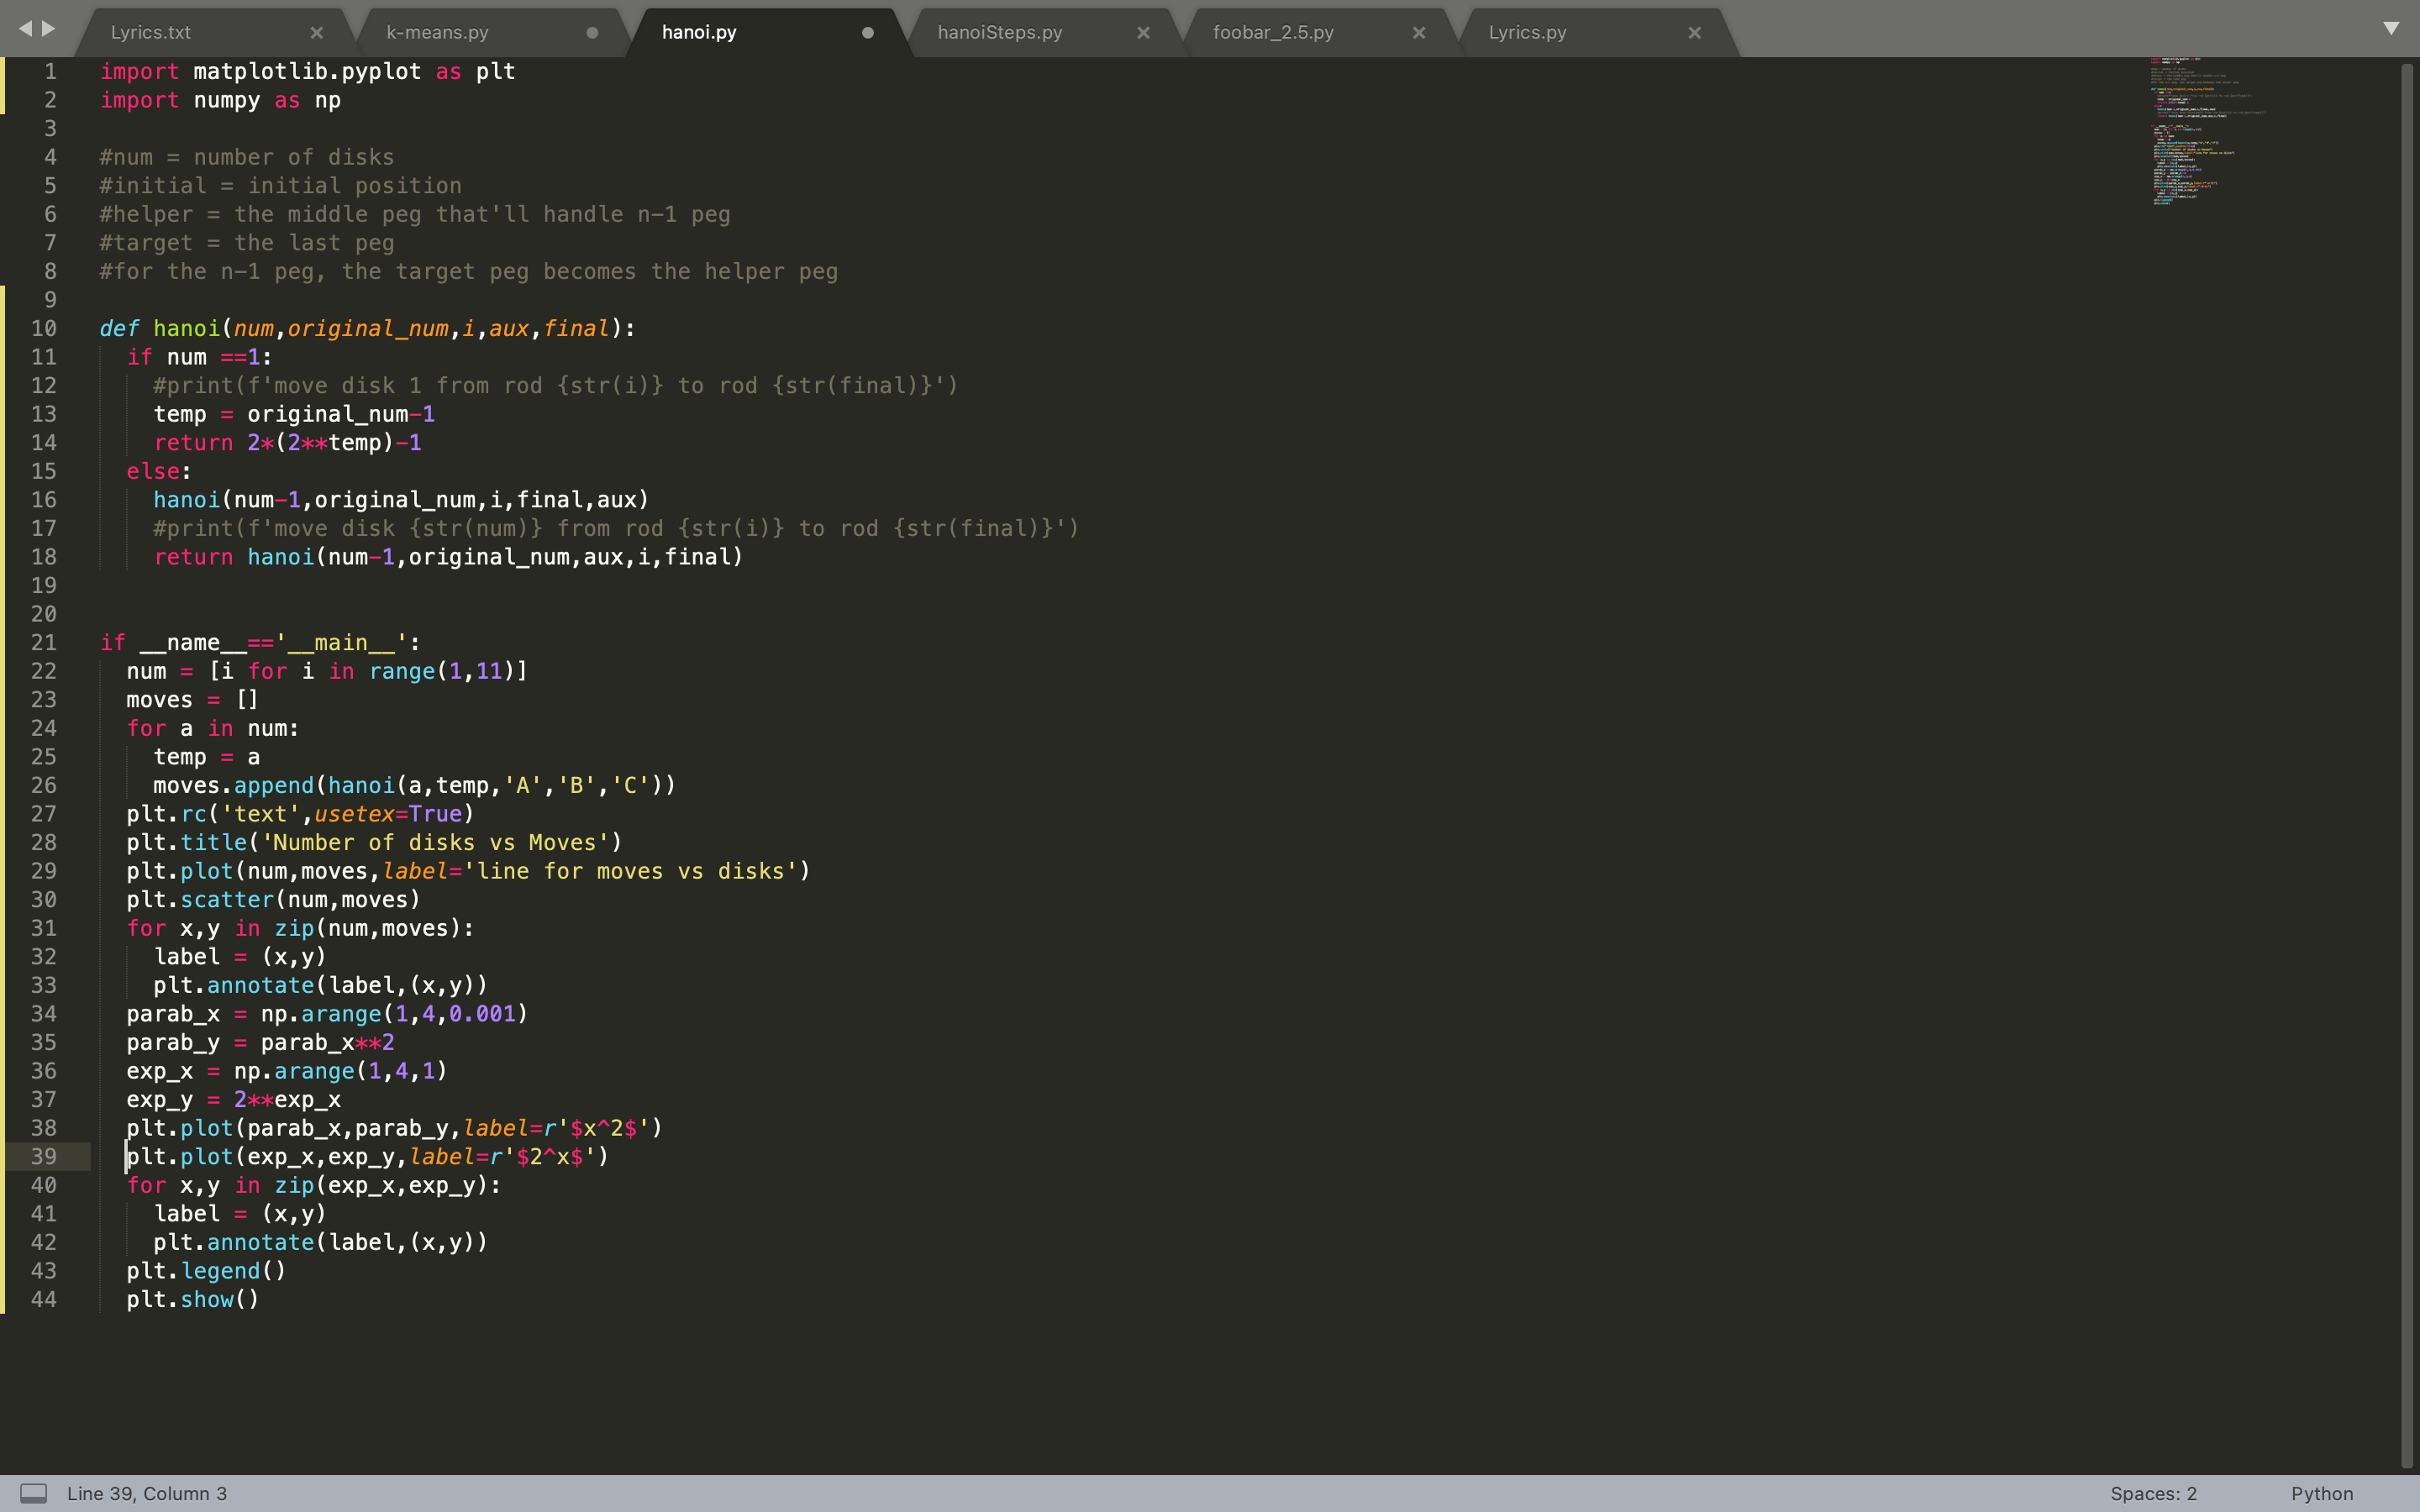
\includegraphics[width=\linewidth]{code_plot.png}
	    \caption{Code to plot the scatter plot, the line over the points, as well as $x^2$ and $2^x$ plots to compare}
	\end{figure}
	\begin{figure}
	    \centering
	    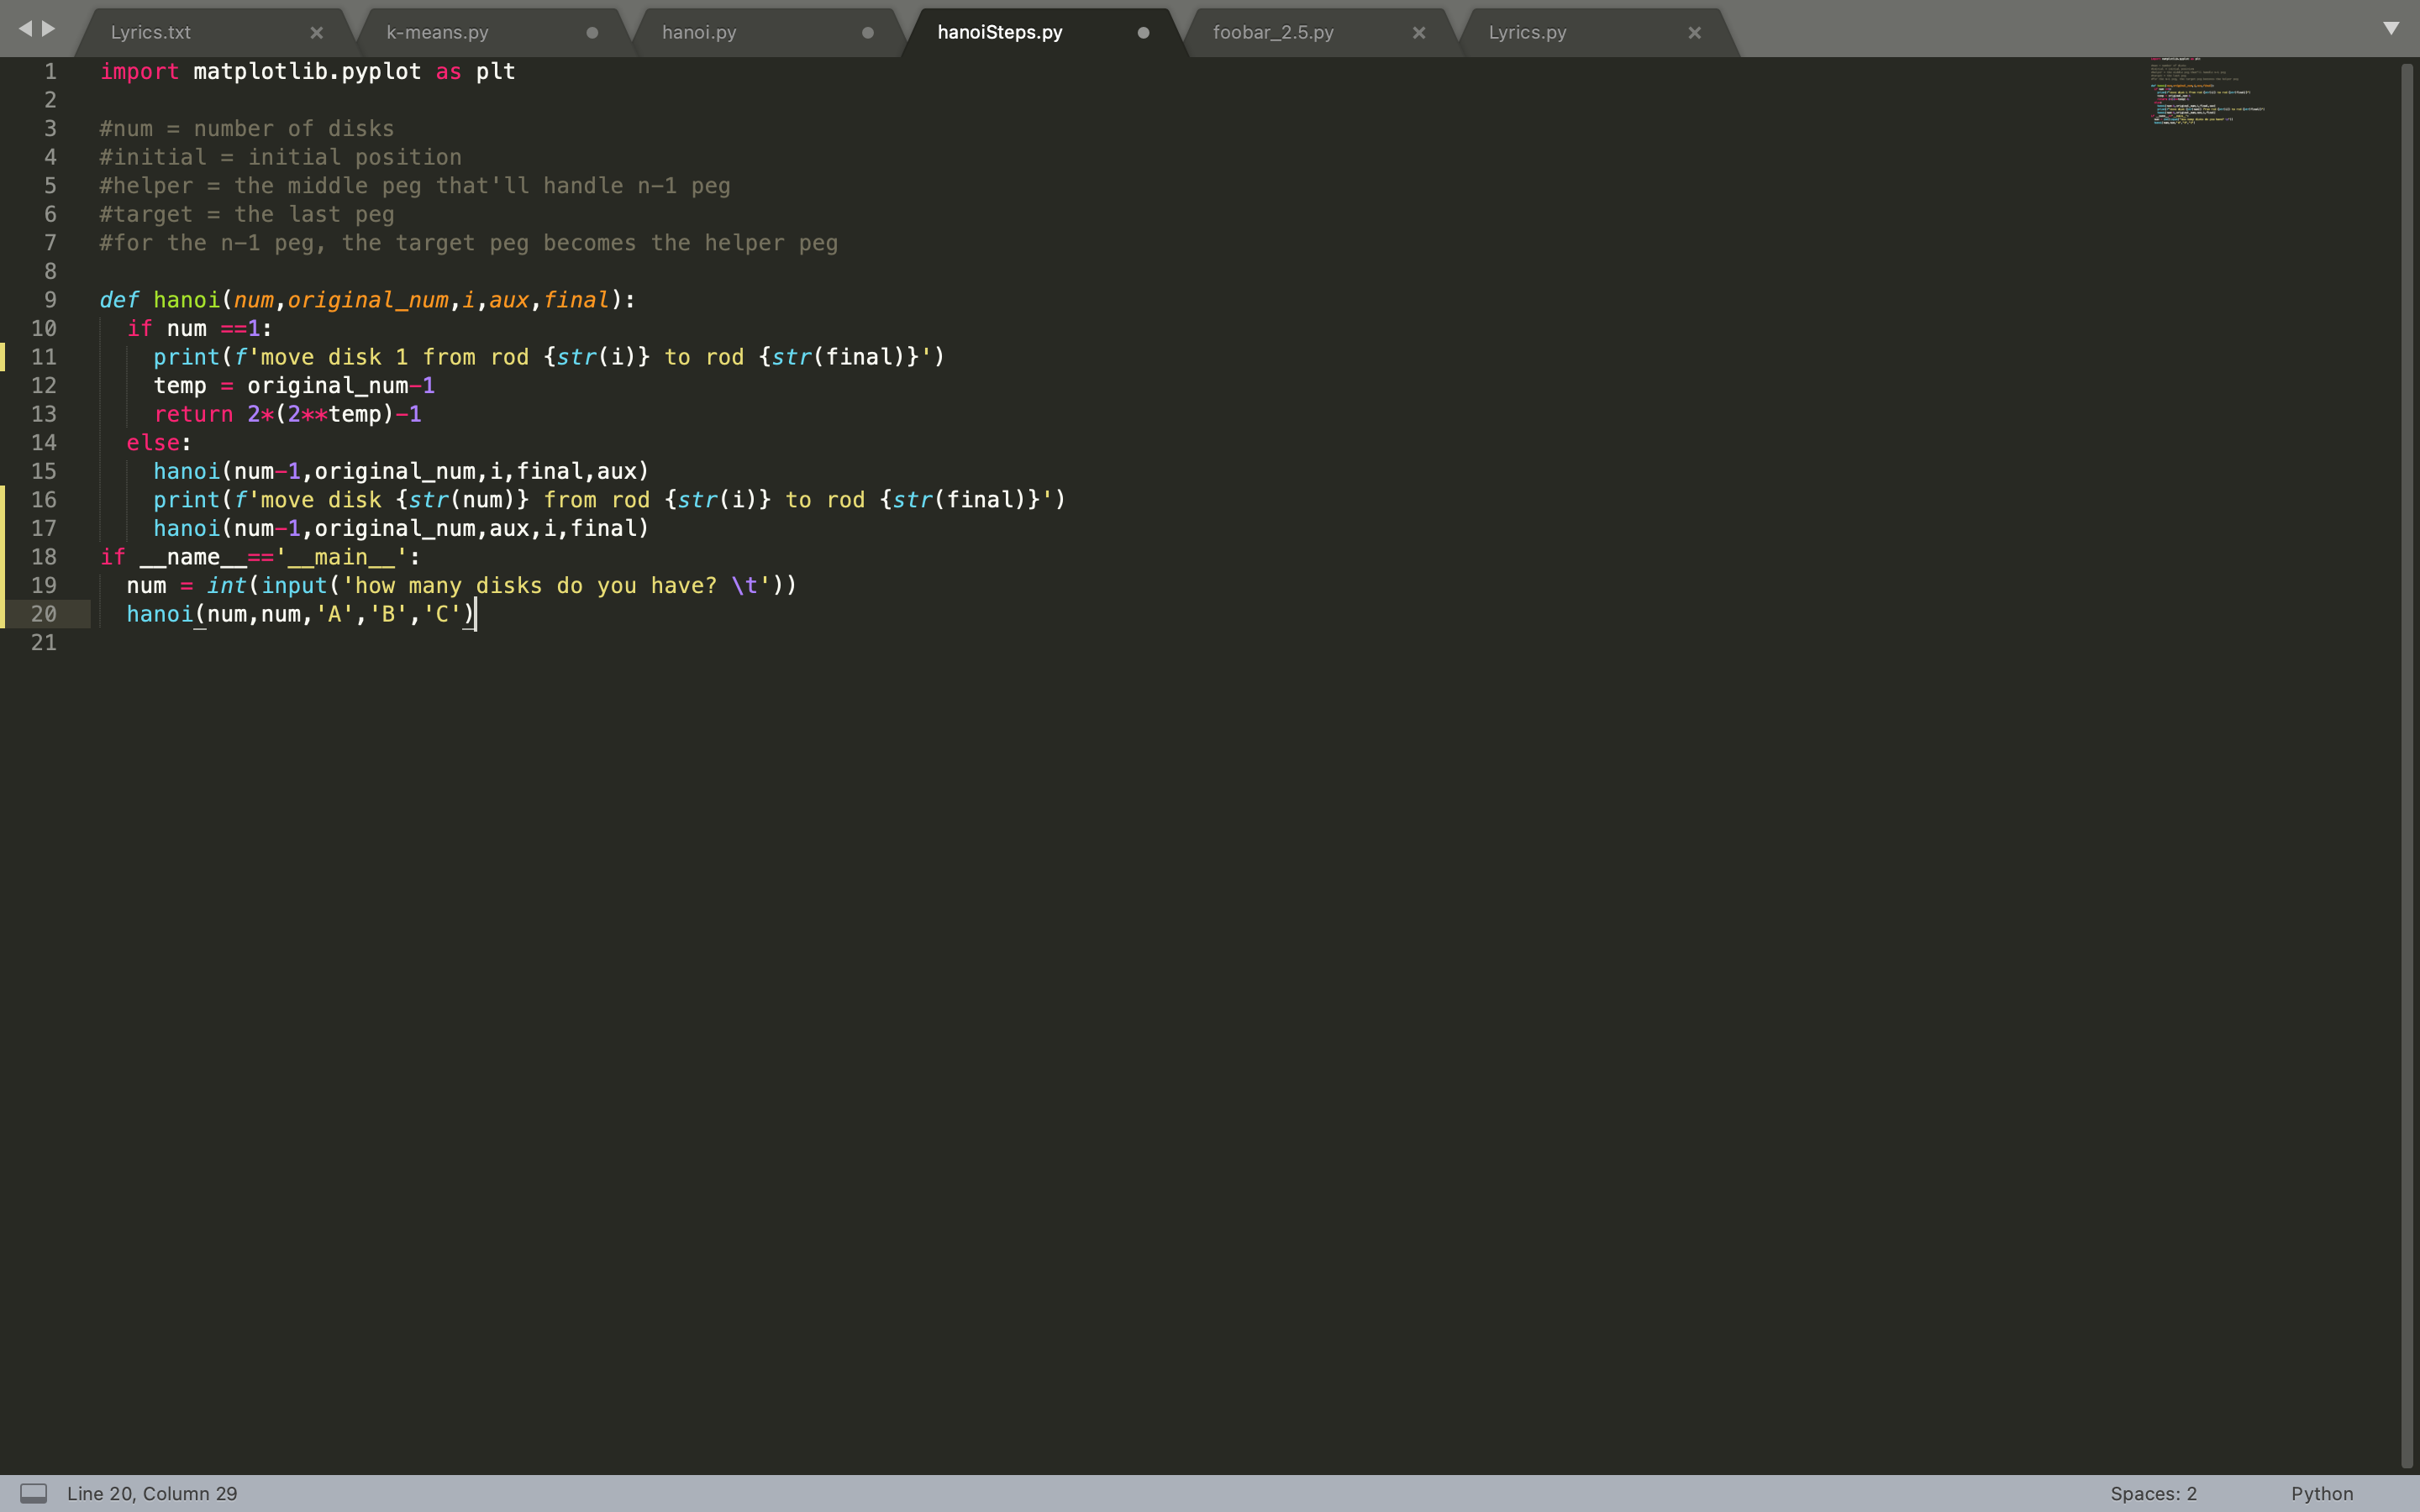
\includegraphics[width=\linewidth]{hanoi.png}
	    \caption{Code to display the steps and ask user how many disk they have}
	\end{figure}
\end{document}
